\documentclass{nime-alternate}
\usepackage{url}
\usepackage{graphicx, color}
\begin{document}

\numberofauthors{1}
\title{Peacock III: The development of an autonomous non-haptic performance instrument}
\author{
\alignauthor
Chikashi Miyama\\
       \affaddr{College of Music and Dance Cologne}\\
       \email{me@chikashi.net}
}

\maketitle
\begin{abstract}
Peacock is a box-shaped instrument for musical performances. Players of this instrument are able to control multiple musical parameters only by moving hands above the instrument. Peacock III, the newest version of Peacock, features a small embedded digital synthesizer, a multi-thread dedicated application, and gesture recognition system. These features enable players to control electronic sound more flexibly and intuitively with the hand gestures.
\end{abstract}

\section{Background}

\begin{figure}[htbp]
       \begin{center}
              \includegraphics[scale = 0.55]{Peacocks.pdf}
       \end{center}
       \caption{Peacock I and II}
       \label{fig:old_peacock}
\end{figure}

Peacock I, the first model of Peacock series, was developed by the author in 2009\cite{miyama:peacock}. It is a musical interface, equipped with 35 infrared proximity sensors that detect the distance between the sensors and the performer's hands. A microcontroller, installed in the interface, collects the data from the sensors, and send them to a host computer. A Pure Data\cite{Pd} patch, running on the host computer, maps the received data from the microcontroller onto the parameters of software synthesizer.

Through five years of musical practice with Peacock I, several points for improvements were discovered:

\begin{enumerate}
\item The bandwidth of the data transfer from the microcontroller to the host computer (ca' 60 Hz.) is not sufficiently high and it causes slight but recognizable latency.

\item The infrared proximity sensors, employed for Peacock I (Sharp GP2D12), detect obstacles in the range only from 10 to 80 cm. This restrict performers from using entire available vertical space above the device. 

\item Since the interface should be connected to a host computer by a USB cable for sound synthesis, a laptop computer must be placed next to the interface. This limits the autonomy and the mobility of Peacock as a musical instrument.

\item The S/N ratio of the analog data from the infrared sensors is not sufficiently high. The data contain significant amount of analog noise and it interferes with the precise paramter control by the hands.

\item The main circuit board of Peacock I is soldered on a single universal board; the cost and labor for the reproduction poses a difficulty in the realization of duo, trio, or ensemble performances with multiple Peacocks.

\item The system currently detects only low-level data from the sensors. By analyzing these low-level data, the detection of hand position and the recognition of hand gestures are possible. These high-level data could be also mapped onto musical parameters and musical commands.

\end{enumerate}

In 2011, this project received a DAAD research scholarship, and Peacock II, a new version of Peacock, was realized at ZKM, Karlsruhe, Germany. The new version solves the first two of abovementioned issues, by employing faster microcontroller\cite{parallax:propeller} and alternative infrared sensors.

\section{Peacock III}

As a solution to the rest of issues, Peacock III, the newest version of Peacock, was designed and realized at Academy of Media Arts, Cologne in 2014.

In order to improve the autonomy and mobility of the device, a small computer for the audio synthesis is embedded in the enclosure of Peacock III. It enables users to play the instrument without connecting it to an external laptop for audio synthesis; Peacock III can be employed as an autonomous electronic instrument, such as electric guitar or keyboard synthesizer. 

Furthermore, a PCB (Printed Circuit Board) is designed as a solution to the fourth and fifth issues. The PCB  denoises the signal from the sensors with hardware lowpass filters, and significantly reduces the cost and labor for the reproduction. 

As a solution for the last issue, a C++ program was developed for gesture recognition; it analyzes the incoming data, detects the hand gestures, and allows us to map the results of the analysis onto musical parameters and commands.

\section{System overview}
\begin{figure}[htbp]
       \begin{center}
              \includegraphics[scale=0.9]{interface_main.jpg}
       \end{center}
       \caption{main unit and interface board}
       \label{fig:interface_main}
\end{figure}

In terms of hardware, Peacock III consists of two components;\\
\textbf{interface board} and \textbf{main unit}. The interface board is a 100mm x 60 mm-sized PCB (printed circuit board), that collects the data from all 35 sensors, digitize them, and forward them to the main unit. It is also equipped with four buttons and a text LCD as a interface for the general system operation.

The main unit, an embeded small computer (102 mm x 102 mm) in the enclosure, analyzes the data from the interface board, maps them onto the parameters of software synthesizers, and generates sound. Optionally, the main unit visualizes the incoming data.

\section{Interface Board} % (fold)

\begin{figure}[htbp]
       \begin{center}
              \includegraphics[width=0.9\columnwidth]{board}
       \end{center}
       \caption{The PCB of Peacock III}
       \label{fig:board}
\end{figure}

The interface board comprises an ATMega 32U2 microcontroller\cite{atmel:avr}, five external 12 bit ADCs, a text LCD, 4 buttons and a Text LCD. The main functionalities of the interface board are as follows:

\begin{enumerate}
       \item stabilization of the sensor power supply by onboard capacitors
       \item digitization of the signal from sensors by 5 ADCs
       \item to provide interfaces for basic operation of the system with the buttons
       \item status indication of the system, using the small LCD
       \item data transfer to the main unit via a USB cable
\end{enumerate}

\begin{figure}[htbp]
       \begin{center}
              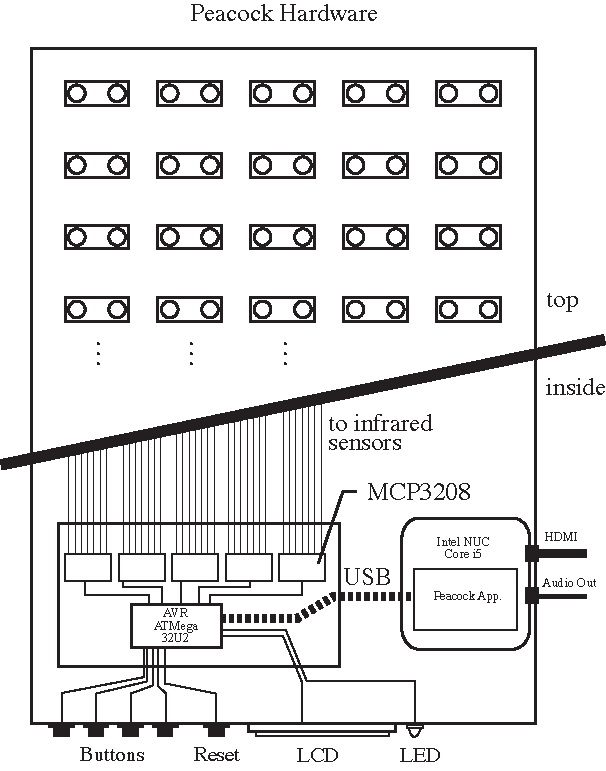
\includegraphics[width=0.9\columnwidth]{Peacock_hardware.pdf}
       \end{center}
       \caption{The Peacock III Hardware}
       \label{fig:peacock}
\end{figure}

\subsubsection{Hardware signal stabilization} % (fold)
The signal from infrared proximity sensors, employed by Peacock, contains significant amount of noise. In the previous version of Peacock, the signal was denoised in the software by applying digital low pass filters to all incoming digital data. However, The PCB of Peacock III is equipped with capcitors for each infrared sensor in order to stabilize its power supply. Since the noise is caused by the rapid current draw that result from pulsations generated by the emitter of the infrared sensors, The stabilization of the power supply removes a significant amount of noise from the analog output signal.

\subsubsection{data collection} % (fold)
In order to collect data from all 35 infrared sensors, five 8 channel 12 bit A/D converters (MCP3208) are installed on the board and they communicates with AVR ATMega 32U2, the main microcontroller on the interface board, using SPI (Serial Periferal Interface) protocol. In the microcontroller, the collected data are packed in 39 bytes-long serial packets, consisting of one byte of start delimeter, end delimeter, message ID, check sum and 35 bytes of actual data from the sensors.

\subsubsection{Status indication/manipulation} % (fold)

A 2x16 text LCD is attached on the side panel of the enclosure and it displays current status of the system. Users are capable of changing the setting of the system, and control the program for the sound synthesis, using buttons, attached next to the LCD.

\subsection{transfer of the data packets} % (fold)

In Peacock I, a FTDI chip bridges the UART messages from the AVR microcontroller to the host computer.
However, by employing AVR ATMega 32U2, a microcontroller with a hardware USB controller, Peacock III is capable of sending data directly from the microcontroller to the host computer. For the development of the USB-compatible firmware, LUFA (Lightweight USB Framework for AVRs)\cite{camera:lufa} was employed. The host computer recognizes the interface board as a virtual serial device and receives data packet more than 1000 time per seconds. 

\section{Main Unit} % (fold)
The Main unit, a dedicated embedded Intel NUC computer\cite{intel:nuc} is placed next to the PCB board in the enclosure. In order to optimize it for musical purpose, it computer runs Arch linux with a realtime kernel.

\subsection{Peacock App}

PeacockApp is an openFrameworks\cite{openframeworks}-based program written in C++. This application receives the data from the interface board and forwards it to the three sub-modules listed below. 

\begin{enumerate}
       \item Gesture Recognizer(PckRecognizer)
       \item Synthesizer(PckSynthesizer)
       \item Visualizer(PckVisualizer)
\end{enumerate}


\begin{figure}[htbp]
       \begin{center}
              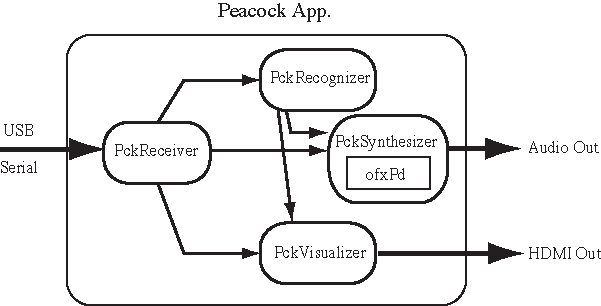
\includegraphics[width=1\columnwidth]{Peacock_app.pdf}
       \end{center}
       \caption{The Peacock III App}
       \label{fig:modules}
\end{figure}

\subsubsection{Gesture Recognizer: PckRecognizer}

The {\it Gesture Recognizer} modules currently detects, the presence and number of hands above the hardware, the estimated position of two hands, and the centroid of each row and column.  If this module find a new gesture, a notification to other two modules will be immediately sent\ref{fig:modules}.

Based on the information of hand positions, this module trances the trajectories of the hands and classifies the gesture. For this end,  SVM (Supported Vector Machine), a common classification algorithm of machine learning was utilized. For the implementation of the algorithm, Gesture Recognition Toolkit \cite{gillian:grt} by Nick Gillian is employed.

\subsubsection{Sound Generator: PckSynthesizer}

The sound generator module is programmed with Pd\cite{Pd}. ofxPd\cite{ofxPd}, an Pd addon for oF\\(OpenFrameworks), enables the PeacockApp to run Pd patches within it. The Pd patches receives all data from the sensors, the result of analysis by the Gesture Recognizer, and the commands from buttons on the side panel. All these data can be mapped to any musical parameters.
 
\subsubsection{Visualizer: PckVisualizer}

Unlike acoustic instruments, players of Peacock controls musical parameters by simply moving hand above the device; There is no physical feedback from the instrument to their hands. In order to train more accurate parameter control by performers, a visualizer for the incoming data was developed.  The visualizer shows the values from 35 infrared sensors, the position of hands, the trajectory of hand movements, and detected gestures in  3D model programmed with OpenGL\cite{OpenGL}. The renderered 3D images can be displayed by attaching an optional HDMI-compatible monitor to the device.
The visualizer can be deactivated by the user, using the attached buttons on the side panel of the enclosure.

In order to minimize the latency and maximize the efficiency of the data processing, these three modules run on three separate threads in PeacockApp. 

\begin{figure}[htbp]
       \begin{center}
              \includegraphics[scale=0.3]{visualizer.png}
       \end{center}
       \caption{Visualizer}
       \label{fig:visualizer}
\end{figure}


\section{future works}

Further improvement of firmware and in the PeacockApp module is scheduled.
The source code of the PeacockApp and Peacock Firmware is hosted on \url{https://github.com/chikashimiyama/Peacock} under GPL v3 lincense.

\section{acknowledgement}
This project is funded by fellowship program of the Academy of Media Arts Cologne. The author would like to express a sincere appreciation to Prof. Anthony Moore and Mr. Dirk Specht for their valuable support.

\bibliographystyle{abbrv}
\bibliography{KHM-references.bib}

\end{document}
